\documentclass{article}

\usepackage{graphicx}
\usepackage{multirow}

\title{Second Generation Sequence Assembly Review}
\author{Sun Zhao}

\begin{document}
\maketitle
\newpage

\begin{abstract}
The abstract abstract.
\end{abstract}

\section{Before Everything}
I would like to first explain the motivation of this article at the beginning. The theme of this article is about sequence assembly which is a computer aided process for constructing gene sequence. It is actually belonging to the scope of bioinformatics. As a pure computer science undergraduate student, I have started researching in this field since the summer in 2010. After reading lots of papers, discussing with biology researchers from China as well as foreign ones, trying kinds of bioinformatic tools, I approached nothing new but valuable experiences of it. In this article, I will answer the questions of "what is gene sequencing", "what is sequence assembly and its challenge", "how to assembly sequence", "how to evaluate sequence assembly softwares" and my own contribution to sequence assembly in a computer science researcher's perspective. I'am not going to tell the deep details but giving initiations about what to do and how to do about sequence assembly. Moreover, I will provide valuable references of related papers and materials to help you get a full view of sequence assembly.
\section{What is gene sequencing}
In genetics and biochemistry, sequencing means to determine the primary structure of an unbranched biopolymer. The biopolymer can be DNA, RNA, protein. In this article, I will focus on DNA and RNA sequence analysis excluding protein. DNA sequencing is the process of determining the nucleotide order of a given DNA chain. Concretely, DNA is a chain of four types nucleotide, represented by letter of `A', `G', `C', `T'. DNA sequencing is trying to produce the corresponding string of `A', `G', `C', `T' for a sample DNA chain. However, the most popular biology sequencing method called shot gun, randomly cut the original DNA chain into fragments and a set of `A', `G', `C', `T' strings. Each nucleotide string which is the sequence of a fragment is called a read. To increase the read coverage and read quality, copies of DNA made by PCR amplification with a typical bacteria template are sequenced. Fig. \ref{shot_gun_method} shows the shot gun process, and you may find that reads are sequenced from the two ends of DNA fragments instead of the complete one. The end sequencing phenomena is caused by biology sequencing methods, however, if particular reaction and methods are included, the distance between the two ends can be estimated. In this case, the two end reads are called pair-end reads and the distance is called insert length.\\
DNA molecules are double-stranded helices, consisting of two long complement strands. According to base paring principle--`A' complements with `T' and `G' complements with `C', the sequence of a strand can be inferred from its opposite one. Particular sequences denoted by 3' and 5' in the DNA strand is used to specify the orientation of the two strand, and for simplicity, if one strand is specified as 3' to 5`, then the opposite one is 5' to 3'.
\begin{figure}[ht]
  \centering
  % Requires \usepackage{graphicx}
  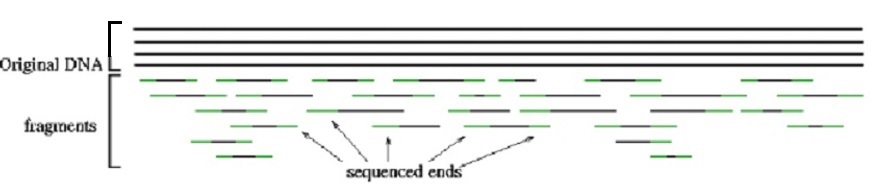
\includegraphics[width=8cm]{Figure1.jpg}\\
  \caption{}\label{shot_gun_method}
\end{figure}

\section{What is sequence assembly}

\end{document}
